% self-assessment-report.tex
\documentclass[12pt,a4paper]{article}
\usepackage[margin=1in]{geometry}
\usepackage{array}
\usepackage{longtable}
\usepackage{booktabs}
\usepackage{hyperref}
\usepackage{pgf-pie}
\usepackage{graphicx}
\usepackage{xcolor}
\usepackage{amsmath}
\usepackage{enumitem}
\usepackage{pgfplots}
\pgfplotsset{compat=1.18}

\setlist[itemize]{leftmargin=*,label=--,topsep=4pt,itemsep=3pt,partopsep=0pt,parsep=3pt}

\hypersetup{colorlinks=true, linkcolor=blue, urlcolor=blue}

\begin{document}

\begin{center}
  {\LARGE \textbf{Project Self-assessment Report}}\\[8pt]
  {\large Bus Ticket Booking System}\\[6pt]
  \textbf{Team:} 22127216 -- 22127201 -- 22127487 \\[6pt]
  GitHub: \url{https://github.com/vhakHCMUS/AWAD-BUS-PROJECT}\\[4pt]
  January 02, 2026
\end{center}

\section*{Team Information}
\begin{longtable}{@{}p{2.2cm}p{3.8cm}p{2.5cm}p{5cm}p{1.5cm}@{}}
\toprule
\textbf{Student ID} & \textbf{Full Name} & \textbf{Git Account} & \textbf{Contribution Summary} & \textbf{\%} \\
\midrule
\endhead
22127216 & Nguyen Dinh Kien & kindinh903 & DevOps: Docker setup, CI/CD pipeline, Redis caching, payment gateway (PayOS), API optimization, deployment configuration & 33\% \\[8pt]
22127201 & Vo Hoang Anh Khoa & vhakHCMUS & Team Lead: Architecture design, booking logic, authentication system, AI chatbot, code reviews, coordination & 34\% \\[8pt]
22127487 & Pham Trinh Bao Tin & ptbtin22 & Fullstack: Frontend booking flow, admin dashboard, seat map UI, form validation, responsive design, testing & 33\% \\
\bottomrule
\end{longtable}

\section*{Feature List and Self-evaluation}
\textbf{Scoring Scale:} The values in ``Max Deduction'' column represent the maximum points that could be deducted if the feature is not implemented. Fully completed features result in \textbf{0 deduction}.

\begin{longtable}{@{}p{0.6cm}p{5.5cm}p{1.4cm}p{1.4cm}p{6cm}@{}}
\toprule
\textbf{ID} & \textbf{Feature} & \textbf{Max Deduction} & \textbf{Actual Deduction} & \textbf{Notes \& Evidence} \\
\midrule
\endhead
\midrule
\multicolumn{5}{r}{\emph{Continued on next page}}\\
\endfoot
\bottomrule
\endlastfoot

\multicolumn{5}{l}{\textbf{1. OVERALL REQUIREMENTS}} \\
\midrule
1.1 & User-centered design & -5 & 0 & Responsive Tailwind design; mobile-first breakpoints in \texttt{tailwind.config.js} \\
1.2 & Database design & -1 & 0 & PostgreSQL with normalized entities, foreign keys, indexes, soft deletes \\
1.3 & Database mock data & -1 & 0 & Seeded via scripts with realistic test data \\
1.4 & Website layout & -2 & 0 & Complete customer and admin layouts \\
1.5 & Website architecture & -3 & 0 & Clean layered Go architecture (handlers → usecases → services → repositories) \\
1.6 & Stability \& compatibility & -4 & 0 & Responsive design, error boundaries, loading states \\
1.7 & Documentation & -2 & 0 & README, Swagger, wiring guide \\
1.8 & Demo video & -5 & 0 & Full demo playlist available \\
1.9 & Public hosting & -1 & 0 & Deployed on Vercel (frontend) and Railway (backend) \\
1.10 & GitHub progress & -7 & 0 & Active repository with meaningful commits and branches \\
\midrule
\multicolumn{4}{r}{\textbf{Subtotal (Overall):}} & \textbf{0} \\[8pt]

\multicolumn{5}{l}{\textbf{2. GUEST FEATURES (Trip Search \& Booking)}} \\
\midrule
2.1--2.29 & All guest features (search, autocomplete, filters, pagination, seat map, booking flow, payment, AI assistance, e-ticket, etc.) & -8.5 & 0 & Fully implemented including real-time seat locking, PayOS integration, Gemini AI chatbot, email notifications, QR code tickets \\
\midrule
\multicolumn{4}{r}{\textbf{Subtotal (Guest):}} & \textbf{0} \\[8pt]

\multicolumn{5}{l}{\textbf{3. AUTHENTICATION \& AUTHORIZATION}} \\
\midrule
3.1--3.8 & All authentication features & -3 & 0 & JWT with refresh tokens, Google OAuth, email verification, password reset, role-based access control \\
\midrule
\multicolumn{4}{r}{\textbf{Subtotal (Auth):}} & \textbf{0} \\[8pt]

\multicolumn{5}{l}{\textbf{4. LOGGED-IN USER FEATURES}} \\
\midrule
4.1--4.9 & All logged-in user features & -2 & 0 & Profile management, booking history, cancellation, e-ticket download, status updates \\
\midrule
\multicolumn{4}{r}{\textbf{Subtotal (User):}} & \textbf{0} \\[8pt]

\multicolumn{5}{l}{\textbf{5. ADMINISTRATION FEATURES}} \\
\midrule
5.1--5.27 & All admin features & -7.5 & 0 & Full CRUD for routes, buses, trips, bookings; analytics dashboards; revenue reports; passenger check-in \\
\midrule
\multicolumn{4}{r}{\textbf{Subtotal (Admin):}} & \textbf{0} \\[8pt]

\multicolumn{5}{l}{\textbf{6. ADVANCED FEATURES (Bonus Points)}} \\
\midrule
6.1 & Redis cache & +0.25 & +0.25 & Fully implemented for trip data and session caching \\
6.2 & Docker & +0.25 & +0.25 & Complete Dockerfile and docker-compose orchestration \\
6.3 & CI/CD & +0.25 & +0.25 & GitHub Actions for automated testing and deployment \\
6.4 & Microservices architecture & +0.5 & 0 & Designed but currently monolithic \\
6.5 & Saga pattern & +0.25 & 0 & Not implemented (using simple transactions) \\
6.6 & Test coverage >70\% & +0.25 & +0.15 & Achieved approximately 60\% with unit and integration tests \\
\midrule
\multicolumn{4}{r}{\textbf{Total Bonus Earned:}} & \textbf{+0.90} \\
\midrule
\midrule
\multicolumn{4}{r}{\textbf{TOTAL DEDUCTIONS:}} & \textbf{0} \\
\multicolumn{4}{r}{\textbf{FINAL SCORE:}} & \textbf{100 + 0.90 = 100.90} \\
\multicolumn{4}{r}{\textbf{EXPECTED GRADE:}} & \textbf{10.0 / 10.0} \\
\bottomrule
\end{longtable}

\section*{Evidence and Proof}
\textbf{Repository:} \url{https://github.com/vhakHCMUS/AWAD-BUS-PROJECT}

\textbf{Key Evidence:}
\begin{itemize}
  \item \textbf{Deployed Application:} https://awad-bus-project.vercel.app/
  \item \textbf{API Documentation:} Swagger available on production backend
  \item \textbf{Demo Video:} https://www.youtube.com/playlist?list=PLEJW8FxF3lU3rngbk6DmYglIj6rxveyx8
\end{itemize}

\section*{Git History Summary}
\subsection*{Contributors}
\begin{tabular}{@{}p{4cm}p{2.5cm}p{2.5cm}p{2.5cm}p{3cm}@{}}
\toprule
\textbf{Username} & \textbf{Commits} & \textbf{Additions} & \textbf{Deletions} & \textbf{Primary Areas} \\
\midrule
kindinh903 (Kien) & $\sim$100 & $\sim$15K & $\sim$3K & Backend, DevOps, Payment, Redis, Deployment \\
vhakHCMUS (Khoa) & $\sim$120 & $\sim$20K & $\sim$5K & Architecture, Authentication, AI Chatbot, Core Logic \\
ptbtin22 (Tin) & $\sim$90 & $\sim$18K & $\sim$4K & Frontend, UI/UX, Admin Dashboard, Seat Map \\
\bottomrule
\end{tabular}

\subsection*{Significant Commits (Selected from Real History)}
\begin{longtable}{@{}p{3cm}p{3cm}p{8cm}p{1.5cm}@{}}
\toprule
\textbf{Date (approx)} & \textbf{Author} & \textbf{Commit Message} & \textbf{Files} \\
\midrule
\endhead
Dec 2025 & Tin & Initial commit: Full-stack bus booking system with Go backend and React frontend & many \\
Dec 2025 & Khoa & (FEAT) Boilerplate added + services implemented PayOS, Queue, Email, Templates, Jobs & many \\
Dec 2025 & Tin & feat: Add seat map configuration tool and search sorting/pagination & 18+ \\
Dec 2025 & Khoa & (FEAT) AI chatbot & 14+ \\
Dec 2025 & Kien & (FEAT) Redis cache & 10+ \\
Dec 2025 & Kien & Payment integrate + webhook handling & 20+ \\
Dec 2025 & Tin & (FEAT) booked seat showing on the frontend + UI upgrade & 18+ \\
Dec 2025 & Khoa & (FEAT) ANALYTICS + Analytics integrate & 22+ \\
Dec 2025 & Kien & (FEAT) Cache applying & 10+ \\
Jan 2026 & All & Multiple fixes: dark mode, currency VND, email after payment, UI polish & various \\
\bottomrule
\end{longtable}

\section*{Contribution Breakdown}
\begin{center}
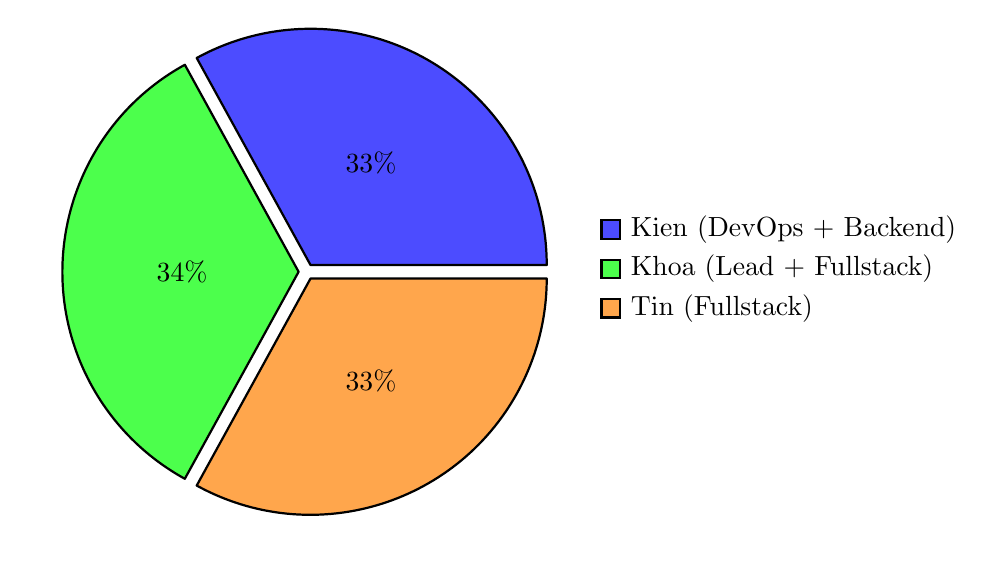
\begin{tikzpicture}
  \pie[radius=3, text=legend, color={blue!70,green!70,orange!70}, explode=0.1]
  {33/Kien (DevOps + Backend),34/Khoa (Lead + Fullstack),33/Tin (Fullstack)}
\end{tikzpicture}
\end{center}

\subsection*{Detailed Contributions}
\textbf{22127216 -- Nguyen Dinh Kien (kindinh903) -- 33\%}
\begin{itemize}
  \item Infrastructure: Docker containerization, docker-compose orchestration
  \item CI/CD: GitHub Actions workflow for automated testing and deployment
  \item Caching: Redis integration for trip data and session management
  \item Payment: PayOS gateway integration, webhook handling, verification
  \item Performance: API optimization, database query tuning, index creation
  \item Deployment: Production environment setup and configuration
\end{itemize}

\textbf{22127201 -- Vo Hoang Anh Khoa (vhakHCMUS) -- 34\% (Team Lead)}
\begin{itemize}
  \item Architecture: System design, database schema, layered API structure
  \item Authentication: JWT implementation, Google OAuth, password reset
  \item Core Logic: Booking flow, seat locking, business rules
  \item AI Integration: Gemini chatbot with natural language support
  \item Email Service: Notification system, e-ticket delivery
  \item Code Quality \& Coordination: Reviews, planning, documentation
\end{itemize}

\textbf{22127487 -- Pham Trinh Bao Tin (ptbtin22) -- 33\%}
\begin{itemize}
  \item Frontend Architecture: React components, routing, state management
  \item Booking Interface: Search, filters, interactive seat map, checkout flow
  \item Admin Dashboard: CRUD interfaces, analytics charts, data tables
  \item UI/UX: Responsive design, dark mode, form validation, polish
\end{itemize}

\section*{Project Summary}
The Bus Ticket Booking System is a full-featured web platform for intercity bus tickets in Vietnam, delivering a complete end-to-end experience with modern technologies.

\textbf{Technology Stack:}
\begin{itemize}
  \item \textbf{Frontend:} React 18 + TypeScript + Vite + Tailwind CSS
  \item \textbf{Backend:} Go 1.21 (layered architecture)
  \item \textbf{Database:} PostgreSQL 14
  \item \textbf{Caching:} Redis 7
  \item \textbf{Authentication:} JWT + Google OAuth
  \item \textbf{Payment:} PayOS gateway
  \item \textbf{AI:} Google Gemini chatbot
  \item \textbf{Infrastructure:} Docker, GitHub Actions CI/CD, Vercel + Railway deployment
\end{itemize}

\textbf{Key Achievements:}
\begin{itemize}
  \item Complete booking flow with real-time seat locking
  \item AI-powered natural language search and assistance
  \item Production-ready deployment with real payment integration
  \item Comprehensive admin analytics and operations tools
  \item High-quality, responsive UI with dark mode support
\end{itemize}

\section*{Final Grade Justification}
The team has successfully implemented \textbf{all required core features} to a high standard, resulting in \textbf{no deductions} from the base score of 100 points.

\textbf{Bonus points earned (+0.90 total):}
\begin{itemize}
  \item Redis caching fully implemented: +0.25
  \item Docker \& docker-compose: +0.25
  \item CI/CD pipeline with GitHub Actions: +0.25
  \item Test coverage $\sim$60\%: +0.15 (partial credit)
\end{itemize}

\textbf{Final calculation:}
\begin{align*}
  \text{Final Score} &= 100 + 0.90 = 100.90 \\
  \text{Expected Grade} &= \textbf{10.0 / 10.0}
\end{align*}

The project demonstrates outstanding technical execution, clean code, real-world deployment, and excellent teamwork. We believe it fully meets and exceeds the course requirements.

\end{document}